\section {Photonik}
\subsection {Grundlagen}
\begin{multicols}{2}
\paragraph {Lichtgeschwindigkeit im Vakuum}
$c = \frac {1}{\sqrt{\mu_0 \epsilon_0}} = 299792458 \frac{m}{s}$

\paragraph {Lichtgeschwindigkeit im Medium}
$c = \frac {1}{\sqrt{\mu_0 \mu_r \epsilon_0 \epsilon_r}}$ auf Leiterplatte $c = 20 \frac{cm}{ns}$ 
\end{multicols}

\paragraph {Photonen}
Licht besteht aus diskreten Energiequanten, den so genannten Photonen.
\begin{multicols}{3}
Energie: \\ $E = h * v$ \\
Plancksche Wirkungsquantum: \\ $h = 6.62606957 * 10^{-34} Js$ \\
Impuls: \\ $p = \frac {h}{\lambda}$ 
\end{multicols}

\subsubsection {Photoeffekt}
\begin{multicols}{4}
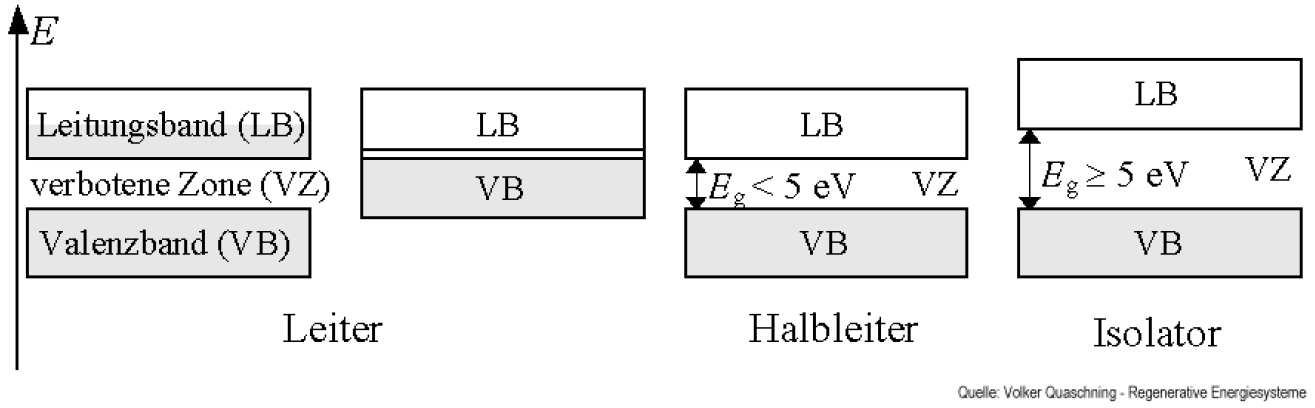
\includegraphics[width=0.5\textwidth]{images/Leitungsband} \\ \columnbreak 
\ \\ \vfill \columnbreak 
Mit der Energie des Lichtes kann ein Elektron auf eine höhere Bahn gehoben werden oder auch herausgeschlagen werden. \\ 
$E = \frac{h * c}{\lambda}$
\end{multicols}

\begin{multicols}{2}
\subsection{Photometrie}
\subsubsection{Empfindlichkeit des Auges}
Bei einer Wellenlänge von 555 nm, einer gelb-grünen Spektralfarbe entsprechend, ist das Auge am empfindlichsten. Bei etwa 510 nm (grün) auf der einen Seite, und bei etwa 610 nm (orangerot) auf der anderen Seite des Maximums erreicht das Auge nur noch die halbe Empfindlichkeit. Bei 665 nm, der Farbe typischer roter Leuchtdioden, beträgt die Empfindlichkeit nur 4,5 Prozent derjenigen bei 555 nm. Bei etwa 380 nm (violett) bzw. 780 nm (tiefrot) ist die Empfindlichkeit fast Null. \\ \\

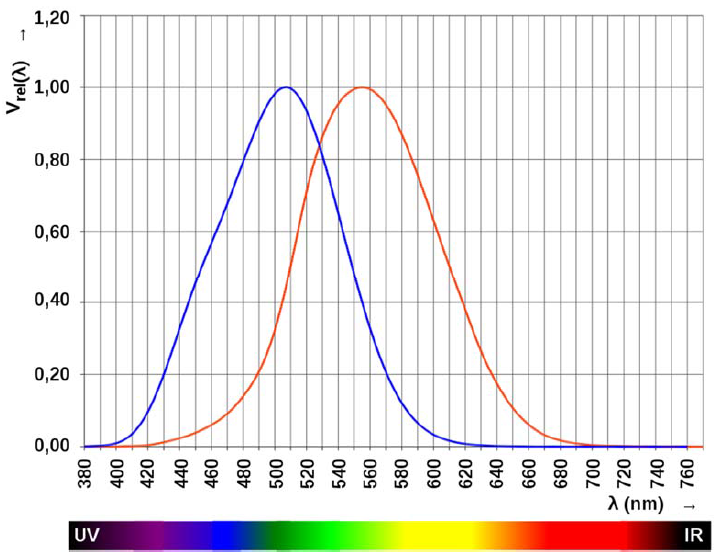
\includegraphics[width=0.4\textwidth]{images/empfindlichkeit_auge} 
\end{multicols}

\subsubsection{Übersicht}
\begin{tabular}{|l|l|l|l|l|l|}
    \hline
    \multicolumn{3}{|l|}{Strahlungsphysikalische Grössen} & \multicolumn{3}{l|}{Lichttechnische Grössen} \\ \hline
    Grösse             & Symbol   & Einheit          & Grösse             & Symbol & Einheit      \\ \hline
    Strahlungsstrom    & $\Phi_e$ & $W$              & Lichtstrom         & $\Phi_v$ & $lm$       \\ \hline
    Strahlstärke       & $I_e$    & $Wsr^{-1}$       & Lichtstärke        & $I_v$    & $cd$       \\ \hline
    Strahldichte       & $L_e$    & $Wm^{-2}sr^{-1}$ & Leuchtdichte       & $L_v$    & $cdm^{-2}$ \\ \hline
    Bestrahlungsstärke & $E_e$    & $Wm^{-2}$        & Beleuchtungsstärke & $E_v$    & $lx$       \\ \hline
\end{tabular}